% !TeX program = xelatex
% Academic block diagrams for the current RV32IM/Zicsr CPU.
\documentclass[tikz,multi=tikzpicture,border=8pt]{standalone}

\usepackage{fontspec}
\setmainfont{Times New Roman}
\setsansfont{Times New Roman}
\setmonofont{Times New Roman}

\usetikzlibrary{
  arrows.meta,
  backgrounds,
  calc,
  fit,
  positioning
}

\definecolor{ink}{HTML}{26384A}
\definecolor{muted}{HTML}{607286}
\definecolor{linegray}{HTML}{AAB6C2}
\definecolor{groupfill}{HTML}{F7F9FB}
\definecolor{frontendfill}{HTML}{E8F1F7}
\definecolor{decodefill}{HTML}{EAF4ED}
\definecolor{executefill}{HTML}{F2ECF8}
\definecolor{memoryfill}{HTML}{FFF2DF}
\definecolor{writebackfill}{HTML}{E9F4F2}
\definecolor{data}{HTML}{356B9A}
\definecolor{memory}{HTML}{C77B24}
\definecolor{control}{HTML}{B84A52}
\definecolor{forward}{HTML}{76519A}

\tikzset{
  font=\rmfamily,
  outer/.style={
    draw=ink,
    rounded corners=2pt,
    line width=0.8pt,
    fill=groupfill
  },
  group/.style={
    draw=linegray,
    rounded corners=2pt,
    line width=0.65pt,
    fill=groupfill
  },
  block/.style={
    draw=ink,
    rounded corners=2pt,
    line width=0.7pt,
    fill=frontendfill,
    align=center,
    text=ink,
    minimum width=2.7cm,
    minimum height=1.15cm,
    inner sep=5pt
  },
  peripheral/.style={
    block,
    fill=memoryfill,
    minimum width=2.7cm,
    minimum height=1.50cm,
    font=\rmfamily\small
  },
  io/.style={
    draw=linegray,
    rounded corners=1.5pt,
    fill=white,
    align=center,
    text=ink,
    minimum width=2.7cm,
    minimum height=0.78cm,
    inner sep=4pt,
    font=\rmfamily\small
  },
  group label/.style={font=\rmfamily\bfseries\small, text=ink, anchor=south west},
  lane label/.style={font=\rmfamily\bfseries\scriptsize, text=ink, anchor=south west},
  datapath/.style={-{Latex[length=2.5mm,width=1.7mm]}, draw=data, line width=1.0pt},
  databoth/.style={{Latex[length=2.3mm,width=1.6mm]}-{Latex[length=2.3mm,width=1.6mm]}, draw=data, line width=1.0pt},
  mempath/.style={-{Latex[length=2.5mm,width=1.7mm]}, draw=memory, line width=1.0pt},
  memboth/.style={{Latex[length=2.3mm,width=1.6mm]}-{Latex[length=2.3mm,width=1.6mm]}, draw=memory, line width=1.0pt},
  controlpath/.style={-{Latex[length=2.4mm,width=1.7mm]}, draw=control, dashed, line width=0.9pt},
  forwardpath/.style={-{Latex[length=2.4mm,width=1.7mm]}, draw=forward, line width=0.95pt},
  bus label/.style={font=\rmfamily\scriptsize, text=muted, fill=white, inner sep=1.5pt, align=center},
  stage/.style={
    draw=ink,
    rounded corners=2pt,
    line width=0.7pt,
    align=center,
    text=ink,
    minimum width=3.05cm,
    minimum height=3.35cm,
    text width=2.72cm,
    inner sep=5pt,
    font=\rmfamily\small
  },
  pipeline register/.style={
    draw=ink,
    rounded corners=1pt,
    line width=0.7pt,
    fill=white,
    minimum width=0.56cm,
    minimum height=7.50cm,
    inner sep=1pt,
    text=ink,
    font=\rmfamily\scriptsize\bfseries
  },
  shared/.style={
    block,
    minimum width=3.4cm,
    minimum height=1.35cm,
    font=\rmfamily\small
  }
}

\begin{document}

% =============================================================================
% SoC hierarchy and interfaces
% =============================================================================
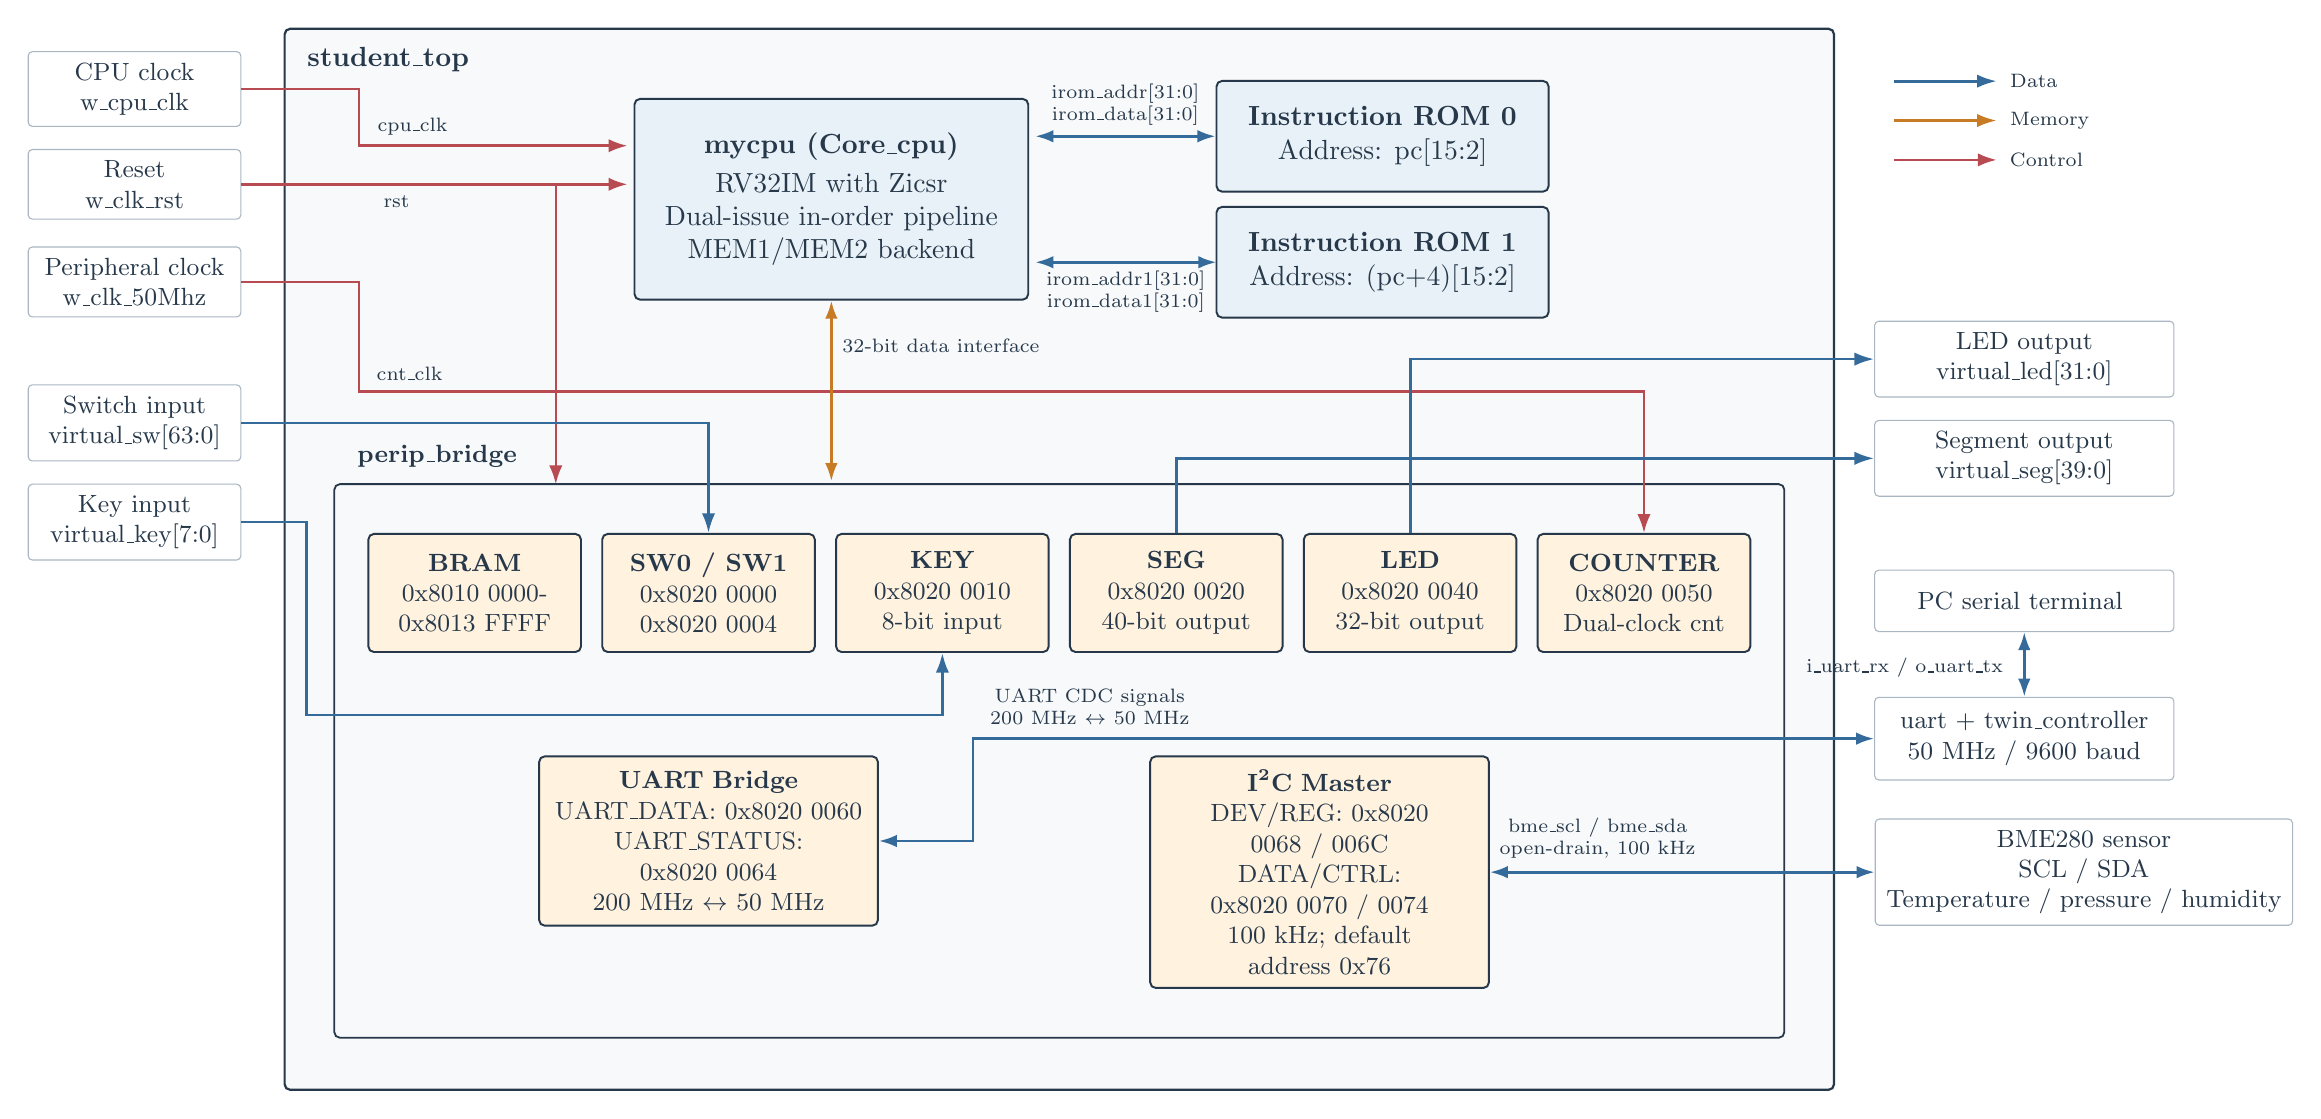
\begin{tikzpicture}[x=1cm,y=1cm]
  % External interfaces
  \node[io] (cpuclk) at (-10.35,6.4) {CPU clock\\w\_cpu\_clk};
  \node[io] (cntclk) at (-10.35,3.95) {Peripheral clock\\w\_clk\_50Mhz};
  \node[io] (reset) at (-10.35,5.19) {Reset\\w\_clk\_rst};
  \node[io] (switches) at (-10.35,2.16) {Switch input\\virtual\_sw[63:0]};
  \node[io] (keys) at (-10.35,0.9) {Key input\\virtual\_key[7:0]};
  \node[io, minimum width=3.8cm] (ledout) at (13.65,2.97) {LED output\\virtual\_led[31:0]};
  \node[io, minimum width=3.8cm] (segout) at (13.65,1.71) {Segment output\\virtual\_seg[39:0]};
  \node[io, minimum width=3.8cm, minimum height=1.05cm] (uarttop) at (13.65,-1.85) {
    uart + twin\_controller\\50 MHz / 9600 baud
  };
  \node[io, minimum width=3.8cm] (pcterm) at (13.65,-0.10) {
    PC serial terminal
  };
  % CPU and instruction memories
  \node[block, minimum width=5.0cm, minimum height=2.55cm] (core) at (-1.50,5) {
    {\bfseries mycpu (Core\_cpu)}\\[2pt]
    RV32IM with Zicsr\\
    Dual-issue in-order pipeline\\
    MEM1/MEM2 backend
  };
  \node[block, minimum width=120pt, minimum height=40pt] (irom0) at (5.5,5.8) {
    {\bfseries Instruction ROM 0}\\Address: pc[15:2]
  };
  \node[block, minimum width=120pt, minimum height=40pt] (irom1) at (5.5,4.2) {
    {\bfseries Instruction ROM 1}\\Address: (pc+4)[15:2]
  };

  % Address-decoded memory and MMIO targets
  \node[peripheral] (bram) at (-6.03,0) {
    {\bfseries BRAM}\\0x8010 0000-\\0x8013 FFFF
  };
  \node[peripheral] (sw) at (-3.06,0) {
    {\bfseries SW0 / SW1}\\0x8020 0000\\0x8020 0004
  };
  \node[peripheral] (key) at (-0.09,0) {
    {\bfseries KEY}\\0x8020 0010\\8-bit input
  };
  \node[peripheral] (seg) at (2.88,0) {
    {\bfseries SEG}\\0x8020 0020\\40-bit output
  };
  \node[peripheral] (led) at (5.85,0) {
    {\bfseries LED}\\0x8020 0040\\32-bit output
  };
  \node[peripheral] (counter) at (8.82,0) {
    {\bfseries COUNTER}\\0x8020 0050\\Dual-clock cnt
  };
  \node[peripheral, minimum width=4.2cm, minimum height=2.15cm,
        text width=3.95cm] (uartbridge) at (-3.06,-3.15) {
    {\bfseries UART Bridge}\\
    UART\_DATA: 0x8020 0060\\
    UART\_STATUS: 0x8020 0064\\
    200 MHz $\leftrightarrow$ 50 MHz
  };
  \node[peripheral, minimum width=4.2cm, minimum height=2.15cm,
        text width=3.95cm, anchor=north] (i2cmaster)
        at ($(uartbridge.north)+(7.76,0)$) {
    {\bfseries I\textsuperscript{2}C Master}\\
    DEV/REG: 0x8020 0068 / 006C\\
    DATA/CTRL: 0x8020 0070 / 0074\\
    100 kHz; default address 0x76
  };
  \coordinate (rightcolleft) at (11.75,0);
  \node[io, minimum width=3.8cm, minimum height=1.15cm, anchor=west] (bme280)
        at (rightcolleft |- i2cmaster.east) {
    BME280 sensor\\SCL / SDA\\Temperature / pressure / humidity
  };

  \begin{scope}[on background layer, xshift=-1pt]
    \node[group, fit=(bram)(sw)(key)(seg)(led)(counter)(uartbridge)(i2cmaster), inner xsep=0.42cm,
          inner ysep=0.62cm] (bridge) {};
    \node[outer, fit=(core)(irom0)(irom1)(bridge), inner xsep=0.62cm,
          inner ysep=0.65cm] (student) {};
    \node[group, fill=none, draw=ink, fit=(bram)(sw)(key)(seg)(led)(counter)(uartbridge)(i2cmaster),
          inner xsep=0.42cm, inner ysep=0.62cm] {};
  \end{scope}
  \node[group label] at ($(bridge.north west)+(0.18,0.08)$) {perip\_bridge};
  \node[font=\rmfamily\bfseries\normalsize, text=ink, anchor=north west]
    at ($(student.north west)+(0.18,-0.12)$) {student\_top};

  % Orthogonal clock and reset paths
  \draw[controlpath, solid] (cpuclk.east) -- (-7.5,6.4) |- node[bus label, above=2pt, fill=none, text=ink, pos=0.6] {cpu\_clk} (-4.09,5.68);
  \draw[controlpath, solid] (reset.east) -- (-7.5,5.19) |- node[bus label, below=2pt, fill=none, text=ink, pos=0.57] {rst} (-4.09,5.19);
  \draw[controlpath, solid] (reset.east) -- (-5,5.19) -- (-5,1.38);
  \draw[controlpath, solid] (cntclk.east) -|(-7.5,2.56)
    -- node[bus label, above=2pt, fill=none, text=ink, pos=0.16] {cnt\_clk} (-3.48,2.56) -| (counter.north);

  % Orthogonal instruction interfaces
  \draw[databoth] (1.09,5.8) -- node[bus label, above=2pt, fill=none, text=ink] {
    irom\_addr[31:0] \\ irom\_data[31:0]
  } (irom0.west);
  \draw[databoth] (1.09,4.2) -- node[bus label, below=1pt, fill=none, text=ink] {
    irom\_addr1[31:0] \\ irom\_data1[31:0]
  } (3.39,4.2);

  % Orthogonal unified data interface
  \draw[memboth] (core.south) -- node[bus label, right=2pt, fill=none, text=ink, near start] {32-bit data interface} (-1.5,1.42);

  % Orthogonal external I/O paths
  \draw[datapath] (switches.east) -| (sw.north);
  \draw[datapath] (keys.east) -| (-8.17,-1.55)
    -- (-0.09,-1.55) -- (key.south);
  \draw[datapath] (led.north) |- (ledout.west);
  \draw[datapath] (seg.north) |- (segout.west);

  % UART path: CPU MMIO -> CDC bridge -> top-level UART/twin -> PC terminal
  \draw[databoth] (uartbridge.east) -- (0.30,-3.15)
    -- (0.30,-1.85)
    -- node[bus label, above=3pt, fill=none, text=ink, pos=0.38] {
      UART CDC signals\\200 MHz $\leftrightarrow$ 50 MHz
    } (4.20,-1.85) -- (uarttop.west);
  \draw[databoth] (uarttop.north) -- node[bus label, left=3pt, fill=none, text=ink, pos=0.45] {
    i\_uart\_rx / o\_uart\_tx
  } (pcterm.south);

  % BME280 path: I2C is independent of KEY and connects only to the sensor
  \draw[databoth] (i2cmaster.east) -- node[bus label, above=3pt, fill=none, text=ink, pos=0.28] {
      bme\_scl / bme\_sda\\open-drain, 100 kHz
    } (bme280.west);

  % Line legend
  \draw[datapath] (12,6.5) -- (13.3,6.5)
    node[bus label, right=1mm, fill=none, text=ink] {Data};
  \draw[mempath] (12,6) -- (13.3,6)
    node[bus label, right=1mm, fill=none, text=ink] {Memory};
  \draw[controlpath, solid] (12,5.5) -- (13.3,5.5)
    node[bus label, right=1mm, fill=none, text=ink] {Control};
\end{tikzpicture}

\end{document}
